\chapter{The Large Hadron Collider and the Compact Muon Solenoid Experiment}
\label{ch:LHC}
	\section{The Large Hadron Collider and other Particle Accelerators}
	Modern experimental particle physics relies on 2 simple ideas, colliding particles together to produce other possibly more interesting or new particles and measuring then measuring these particles directly or measuring their decay products in a large multipurpose detector. Over the years, a large number of experiments have been involved in discovering and confirming most of the particles and properties in the standard model. They have followed a general trend of using either leptons or hadrons to exploit various theoretical properties to produce certain particles more readily, or ratcheting up the center of mass energy of the collisions from the previous similar experiment (see Figure~\ref{fig:experiment_energies}) or increasing the rate of collisions in order to collect more data more quickly. Most new experiments rely on some combination of all of these methods to improve over the previous ones and open up new areas of exploration.\\
	
		\begin{figure}[h]
\begin{center}

\includegraphics[width=0.48\linewidth]{Figs/placeholder.pdf}
\caption{\label{fig:experiment_energies}
Plot of various experiments, their energies and famous discoveries ~\cite{}.
}
\end{center}
\end{figure} 
	
	The Large Hadron Collider (LHC) is the worlds current largest and most powerful particle accelerator ~\ref{http://home.web.cern.ch/topics/large-hadron-collider}. It is situated at the European Organization for Nuclear Research (CERN) which is headquartered in Geneva, Switzerland, but crosses the border into France (see Fig.~\ref{fig:cern_map}). The machine first started up on September 10 2008 and has collected data periodically since then. The LHC is housed in a 27 km long ring buried underground in which 2 beams of protons circulate at near the speed of light in opposite directions (see Fig.~\ref{fig:lhc_beampipe}). The majority of this ring is filled with superconducting electromagnets to guide the beams, equipment to super cool the magnets to $-271.3^\circ$~C and hold the beam pipes at an ultrahigh vacuum, and other odds and ends to keep the beam circulating. There are 1232 dipole magnets each 15 metes in length to bend the beams and 392 quadrupole magnets  each 5-7 meters in length to focus the beams. By focusing the beams, particles are not lost while circulating and the rate of collision of passing bunches is increased.
	
				\begin{figure}[h]
\begin{center}

\includegraphics[width=0.48\linewidth]{Figs/placeholder.pdf}
\caption{\label{fig:lhc_beampipe}
Map of CERN including LHC ring ~\cite{}.
}
\end{center}
\end{figure} 
	
			\begin{figure}[h]
\begin{center}
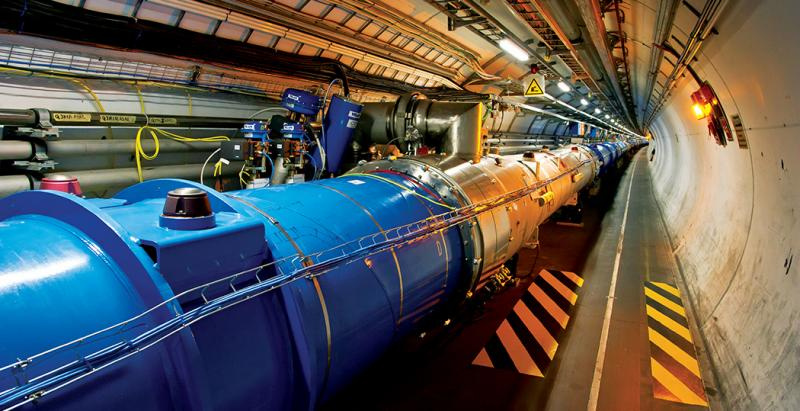
\includegraphics[width=0.48\linewidth]{Figs/lhc_beampipe.jpg}
\caption{\label{fig:lhc_beampipe}
Picture of the interior of the LHC showing the beam pipe and some equipment. Particles circulate around the ring in the very center of this pipe (which is mostly filled with electronics) ~\cite{http://home.web.cern.ch/topics/large-hadron-collider}.
}
\end{center}
\end{figure} 
			
	
	
	\section{Description of CMS detector}        
		The LHC collides protons over 40 million times a second. Most of these are glancing blows, but some are direct collisions that convert some of the extreme energy in the proton momentum into heavy short lived particles that do not usually exist naturally on Earth. The Compact Muon Solenoid (CMS) is one of a few detectors situated at one of the collision spots at the LHC designed to measure the properties of these heavy short lived particles and their decay products. Because of the wide range of heavy particles and decay products, CMS is a general purpose detector, designed to measure momentum, energy, charge, and other properties of many different light particles from quarks to leptons to hadrons. The CMS detector is composed of a number of layers that each perform a different role in measurement and combined can paint a very detailed picture of a wide variety of physical phenomena and can be used to reconstruct an entire collision and resulting decays.\\
		
\begin{figure}[h]
\begin{center}
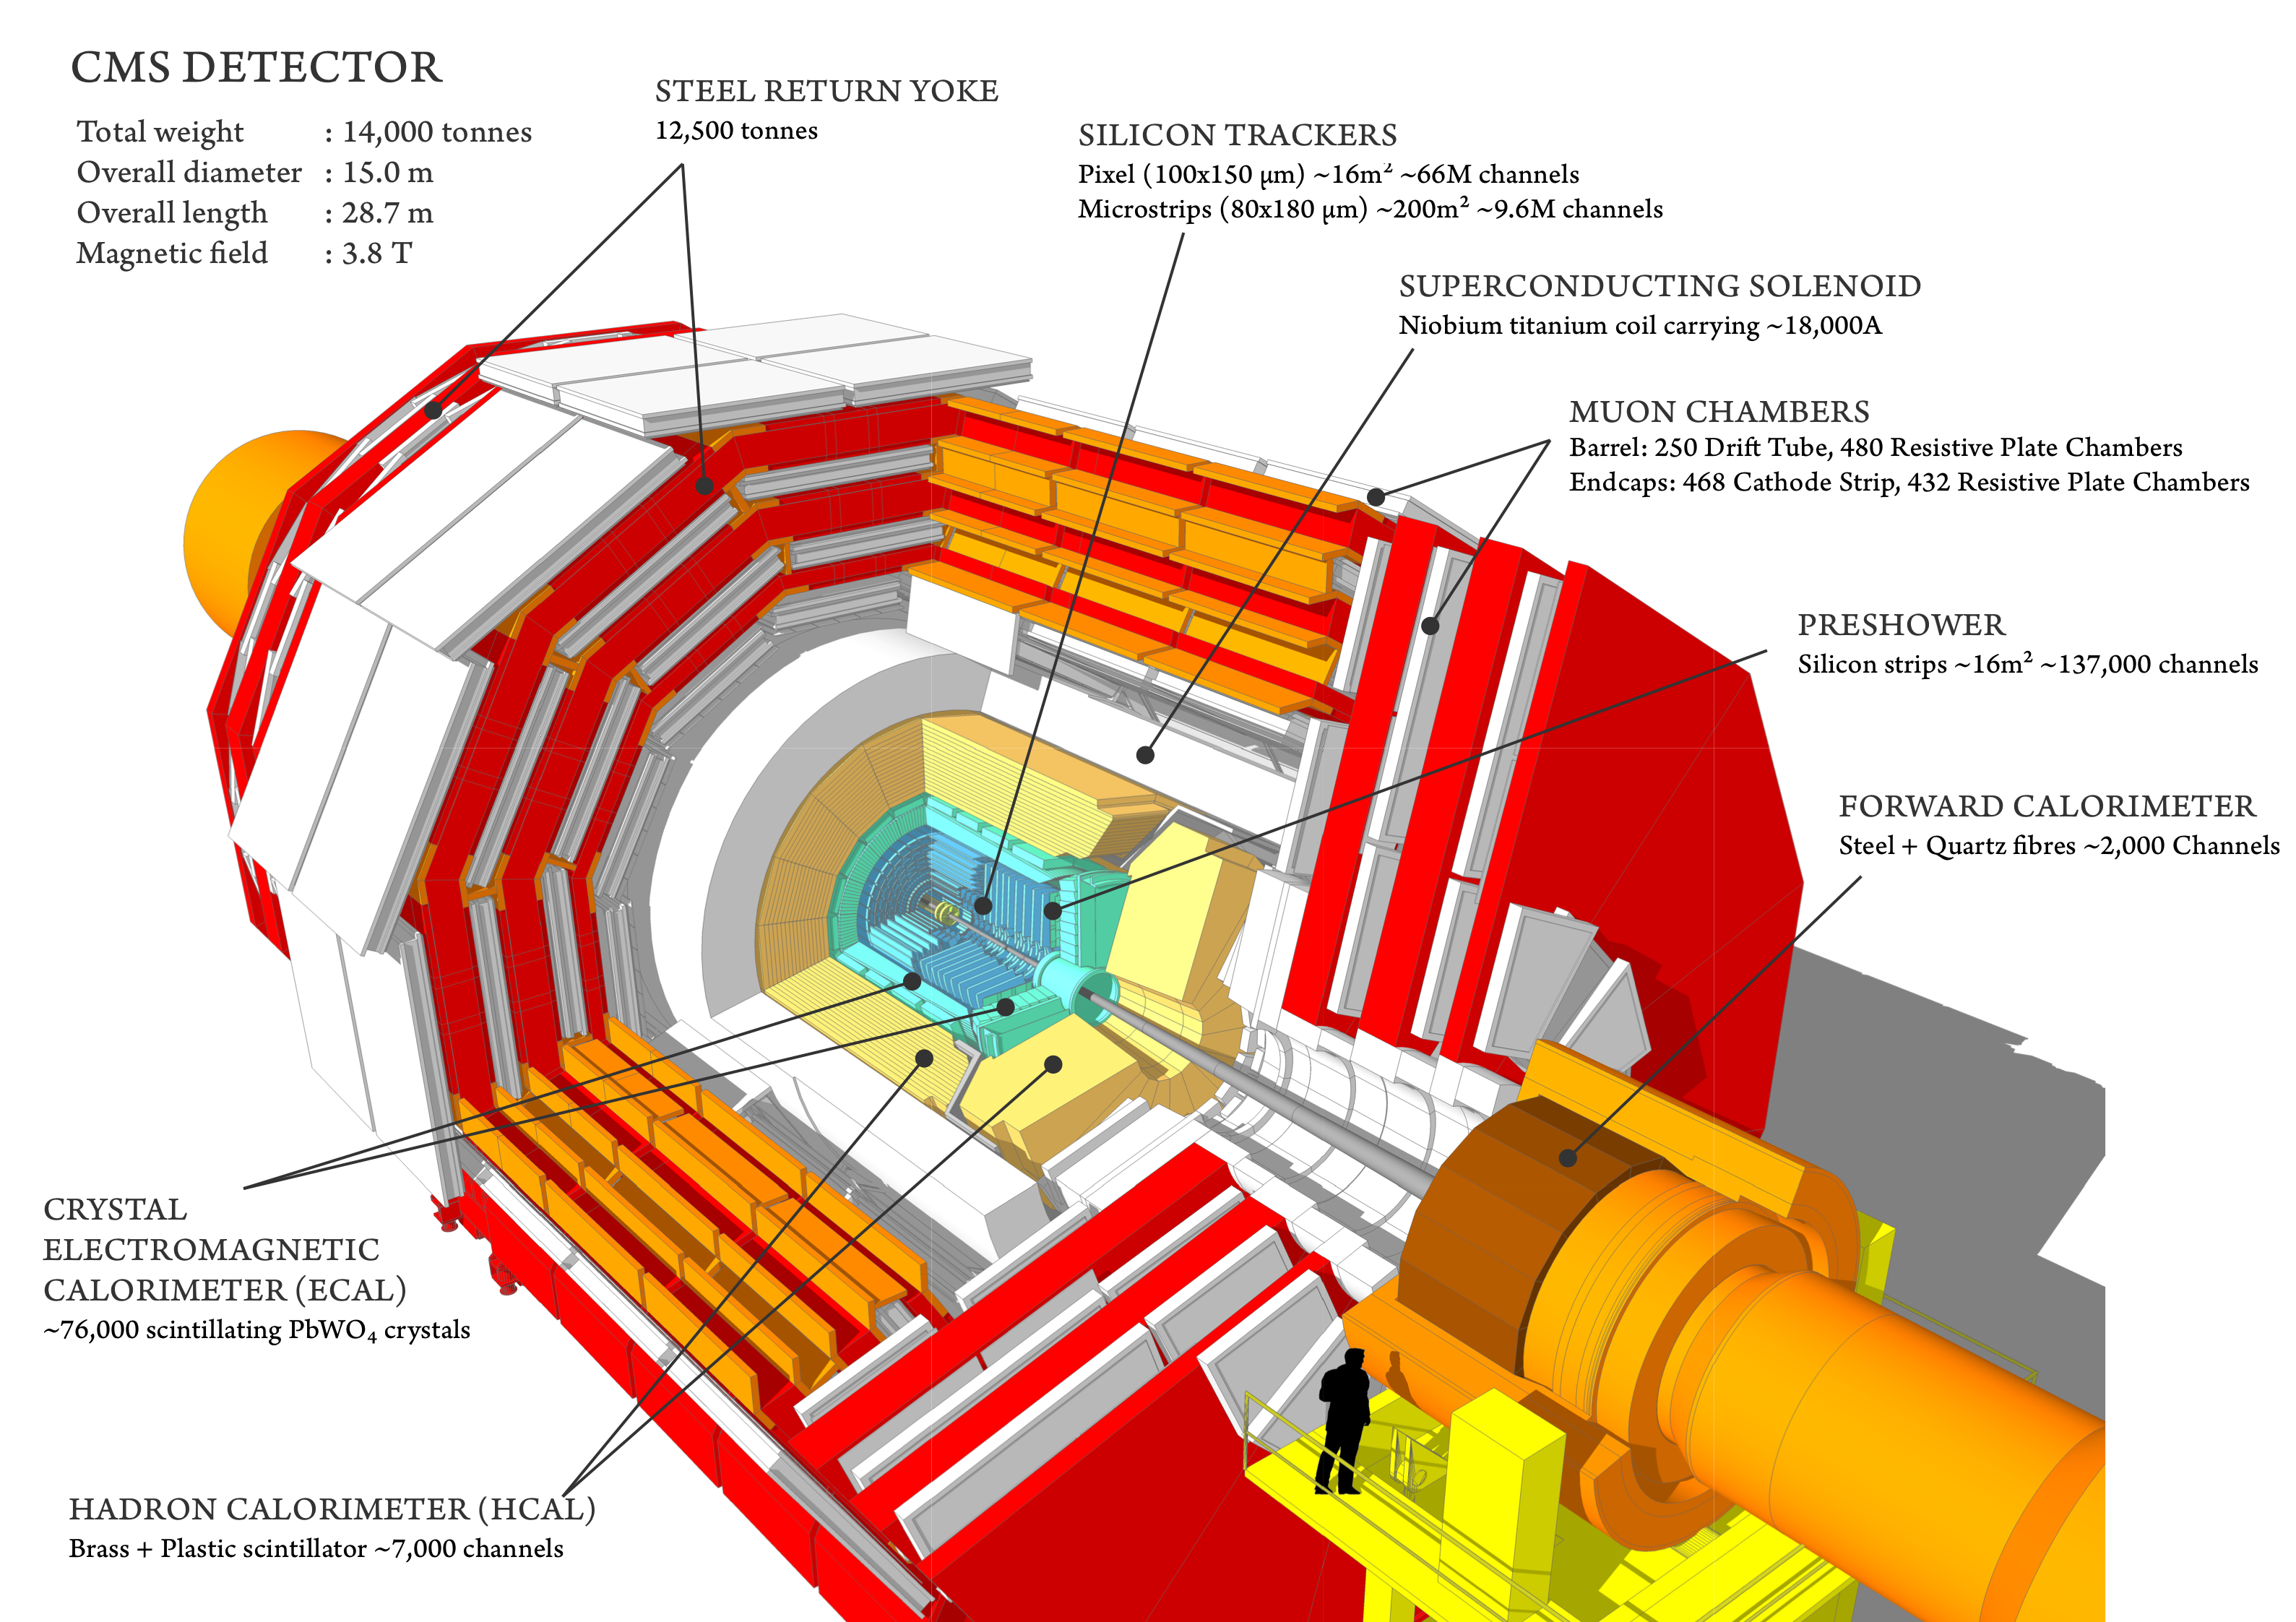
\includegraphics[width=0.48\linewidth]{Figs/cms_detector_internal.png}
\caption{\label{fig:cms_slice}
The CMS detector opened up so all layers are visible ~\cite{http://cms.web.cern.ch/news/cms-detector-design}.
}
\end{center}
\end{figure} 

		
\begin{figure}[h]
\begin{center}
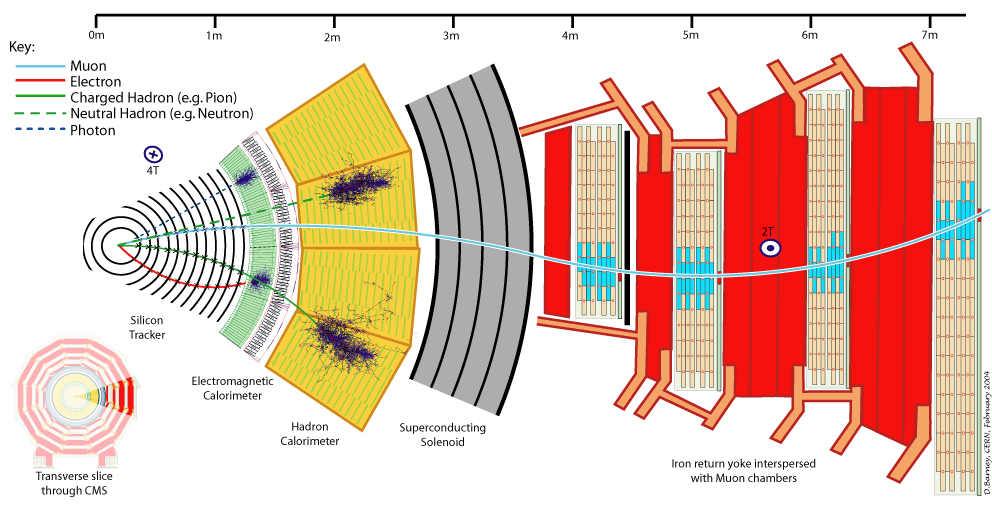
\includegraphics[width=0.48\linewidth]{Figs/CMS_Slice.png}
\caption{\label{fig:cms_slice}
Picture of a cross sectional slice of the CMS detector ~\cite{https://cms-docdb.cern.ch/cgi-bin/PublicDocDB/ShowDocument?docid=4172}.
}
\end{center}
\end{figure} 

The CMS detector design strives to achieve the following:
\begin{itemize}
\item A high performance system to detect and measure muons (see Muon Detector ~\ref{sec:muon_detector}).
\item A high resolution system to measure the energy and showering shape of electrons and muons (see Electromagnetic Calorimeter ~\ref{sec:electromagnetic_calorimeter}).
\item A high quality system to measure the trajectory of charged particles for accurate momentum measurements (see Silicon Tracker~\ref{sec:silicon_tracker}).
\item A hermetic system that surrounds the collision and fully measures the complete hadronic energy of the event (see Hadronic Calorimeter~\ref{sec:hadronic_calorimeter}).
\item A strong magnetic field to curve the charged particles' trajectories to aid in momentum, energy, and mass measurements as well as identification of the particles' spatial origins (see Solenoidal Magnet~\ref{sec:solenoidal_magnet}).
\end{itemize}

	\subsection{Solenoidal Magnet}
	\label{sec:solenoidal_magnet}
The CMS detector uses a fundamental physical property to help measure momentum: a charged particle's trajectory curves when it travels in a magnetic field. The magnet is a solenoid and just has a field along the Z-axis causing particles to curve in the xy-plane. The solenoid is 13 m long and 7 m in diameter which allows for most of the electronics to be placed inside it. The solenoid is made of a coil of superconducting wire that runs with above  18,000 A of current to create a 3.8 T field storing 2.3 GJ of energy. It is the strongest magnet of it's kind in the world. The magnet strength was chosen to be low enough to allow electrons and other charged particles produced at the lower range of interesting energy to escape the tracker (too strong a field would cause them to curl around inside the tracker) and large enough that very high energy particles still travel with enough curvature that the tracker can somewhat accurately measure the curvature and thus momentum.		
		
					\begin{figure}[h]
\begin{center}

\includegraphics[width=0.48\linewidth]{Figs/placeholder.pdf}
\caption{\label{fig:magnet}
.
}
\end{center}
\end{figure}

	\subsection{Silicon Tracker}
	\label{sec:silicon_tracker}
	The silicon tracker is discussed as a single measurement device, but is actually made up of two different arrangements of silicon detectors. The inner area which is closest to the collision and will contain the highest density of particles and thus points of measurement is made out of silicon pixels measuring 100\um by 150 \um. This section also receives the highest dosage of radiation of any of the detector components and must be extremely resilient to radiation. There are 65 million channels of pixels, and thus power consumption was kept to a minimum at 50 microwatts a channel. Even so, the pixels are mounted on cooling tubes so as not to overheat the detector. The silicon tracker exploits a property of silicon where charged particles eject electrons from the silicon atoms as the particles traverse the silicon. Each pixel collects these charges on the surface and measures them as a small electric signal. \\
	
	The outer layer of the tracker does not quite need this level of precision and instead of having pixels, uses more granular "strips" of silicon. This lowers the cost of producing the silicon and even more importantly lowers the amount of readout channels required. Some extra precision is picked up by angling overlapping layers of strips (10 in total) slightly off of parallel to provide a level of stereoscopic location. Thus a rough estimate of which part of a strip the particle passed through can be made by looking at which strip it hit on the next layer.\\
	
	The Silicon strips make up four inner barrel layers with two inner end caps, 6 outer barrel layers, and 2 outer end caps. The end caps make the pixel detector hermetically sealed, but do not provide the same precision as the barrel track do to a lack of pixels. Thus most charged particles tend to only considered strongly identified and have well reconstructed momentum if they are picked up by the barrel tracker.\\
	
						\begin{figure}[h]
\begin{center}

\includegraphics[width=0.48\linewidth]{Figs/placeholder.pdf}
\caption{\label{fig:tracker}
.
}
\end{center}
\end{figure}
	
	\subsection{Electromagnetic Calorimeter}
	\label{sec:electromagnetic_calorimeter}
	Once a particle's trajectory has been measured in the tracker (with minimal energy loss), it is time to measure the particles total energy as well. This step must be done second as measuring the energy of a particle is messy requiring collisions with a material that will alter and stop the particle's movement. The CMS detector additionally exploits the fact that different particles interact with different material at different rates. Thus a calorimeter can be designed to primarily measure the energy of electromagnetic particles such as electrons and muons while letting hadronic particles (quarks) mostly pass through to the next layer. This helps both with energy measurement as well as identification. At a very reduced level of complexity, electrons have a track in the tracker and leave a large amount of energy in the Electromagnetic Calorimeter (ECAL) and little to no energy in the Hadronic Calorimeter (HCAL). Photons are similar but being neutral do not leave tracks. Quarks, charged mesons, and jets have tracks and leave some energy in the ECAL and deposit the majority of the energy in the HCAL (see Section ~\ref{sec:hadronic_calorimeter}).\\
	
	The ECAL is made of lead tungstate (PbWO4) crystals that are very dense. With oxygen added into the crystals, they are relatively transparent to light, and scintillate (release a large amount of photons) when an electron or photon pass through them. This scintillation is immediate, short lived, and well defined by the incoming particle's energy. Thus the ECAL is compact and accurate at measuring energy at the frequency of collisions at the LHC. In the barrel, the crystals measure 2.2 x 2.2 x 23 cm and 3 x 3 x 22 cm in the end caps with a total of 75,848 crystals in the ECAL. There is additionally a pre shower system which helps crudely measure the trajectory of the particles after leaving the tracker (useful for determining the photon trajectory and matching electron showers to tracks).\\
	 
	 Mollier radius?
	 
						\begin{figure}[h]
\begin{center}

\includegraphics[width=0.48\linewidth]{Figs/placeholder.pdf}
\caption{\label{fig:ecal}
.
}
\end{center}
\end{figure}
	
	\subsection{Hadronic Calorimeter}
	\label{sec:hadronic_calorimeter}
	The Hadronic Calorimeter (HCAL) uses a different set of materials with different interaction properties to stop and measure the energy of hadronic particles which are made of quarks and gluons. This layer is outside the ECAL and thus measures very little energy from electromagnetic particles such as electrons and muons. The HCAl is hermetically sealed so that it should measure all of the energy in the collision that has not already been measured by the ECAL. Notable exceptions include muons which get measured in the Muon Chamber and weakly interacting neutral particles such as neutrinos (or possible Super Symmetric particles). The later weakly interacting particles can be inferred by a momentum and energy imbalance thanks to the hermetic properties of the detector and the conservation of energy.\\
	
	The HCAl is a sampling calorimeter structured with alternating layers of absorbing material  which causes incoming particles to shower and scintillators which produce light when the showers pass through. The scintillator light is amplified by photodetectors. Each layer can record position, energy, and time of arrival. Sections of radial layers are grouped together to form a ``tower," and the towers are used to determine the total energy and the direction of travel of the particle that produced it by grouping energy filled towers together that are near each other.\\
	
	The overall HCAL consists of a barrel section assembled from 36 wedges, an endcap section also made of 36 wedges, and forward sections which pick up particles that come out at very shallow angles to the beam line.
	
						\begin{figure}[h]
\begin{center}

\includegraphics[width=0.48\linewidth]{Figs/placeholder.pdf}
\caption{\label{fig:hcal}
.
}
\end{center}
\end{figure}
	
	\subsection{Muon Detector}
	\label{sec:muon_detector}
	Muons are charged leptons like electrons, so they leave a track in the tracker. Unlike electrons, muons interact somewhat weakly and thus do not shower in the ECAL. Because of their ability to pass through several meters of iron, there is a special section to measure muons which is placed on the outside of the detector after all of the other particles should have showered and been stopped by the two calorimeters and the iron return yoke.\\
	
	The muon detector consists of 4 layers each divided into smaller modules known as ``stations." The layers are separated by iron which is part of the return yoke. Because the muon detector is located outside of the solenoid, the return yoke helps to create a magnetic field in the opposite direction of the field inside the solenoid, thus when the Tracker and Muon Detector show the trajectory of a muon, it looks like an 'S.'\\
	
	Within the Muon Detector, there are 1400 chambers: 250 drift tubes (DTs), 540 cathode strip chambers (CSCs) (for position measurements and triggering), and 610 resistive plate chambers (RPCs) (as a redundant triggering system). The DTs and RPCs are arranged in concentric cylinders around the beam line while the CSCs and RPCs make the disks that cover the ends of the cylinder.\\
	
	The Muon Drift Tubes are 4 cm wide tubes which contain a wire stretched down the length of the tube and a gas that is prone to losing electrons as charged particles pass through it. A voltage is applied across the wire and thus knocked off electrons are collected at the positive end. Using the amount of charge collected, the distance of closest approach to the wire can be calculated. Using the amount of time it takes to move the charge down the wire to the positive end, the distance position along the wire's access can be determined for the muon's approach. Thus each tube can give a 2 dimensional position measurement of the muon. To make a DT chamber, 60 DTs are collected into 12 layers arranged in 3 groups of 4. The DT chambers average 2mx2.5m in size and multiple DT chambers surround the detector.\\
	
	The CSCs are composed of overlapping and perpendicular copper cathodes and anode wires. Between the two layers is a gas. Electrons from the gas are collected on the anodes and ions (now missing an electron) are collected on the cathodes. This a very fast system and thus is suitable for triggering. RPCs work similarly but instead have two parallel plates made of a highly resistive material. Strips outside the plates pick up the presence of the charged particles. RPCs have good spatial resolution and time resolution down to 1 nanosecond which also makes them excellent for triggering.\\
						\begin{figure}[h]
\begin{center}

\includegraphics[width=0.48\linewidth]{Figs/placeholder.pdf}%muonstations.gif, muonDriftTube.gif
\caption{\label{fig:muonchamber}
.
}
\end{center}
\end{figure}
	
		
		
	
	\section{Luminosity Measurement}	
		Luminosity is defined as the ratio of the number of particles detecte (N) in a certain time (t) to the interaction cross-section ($\sigma$). 
		\begin{equation}
		\mathcal{L} = \frac{1}{\sigma} \frac{dN}{dt}
		\end{equation}
		
		The relationship between luminosity, cross section, and number of collisions was expressed early in another form in Equation ~\ref{eq:lumi_xsec_relationship}. The form above expresses the luminosity in terms of an instantaneous value whereas the useful form for particle physics is integrated luminosity, which as the name implies is the total luminosity over time and not just at any given instant. Luminosity can be thought of conceptually in a naive analogy with light. If one turns on a light in a room, there is some level of luminosity which correlates to the number of photons per second leaving the light bulb. The more luminosity the bulb provides, the more light will scatter off of objects and return to the person's eye and the better the person can see the surrounding area. In particle physics, luminosity correlates to the amount of collisions that can be produced with any given cross section. If one provides fixed objects (such as protons) then the cross section is also fixed, and thus the only way to increase the number of collisions is to increase the luminosity, which among other things depends highly on the number of particles passing in close proximity to each other per unit time. \\
		
		Up to the end of data taking in 2012, the LHC delivered an integrated luminosity of 23.3 \fbinv. Of collisions produced, CMS was able to record 21.8 \fbinv and due to various transient issues, was able to certify 19.5 \fbinv of integrated luminosity as ``good" data that could be used for measure physical phenomena. The uncertainty on this measurement was 4.4\% ~\cite{} and contributes to the total uncertainty of any measurement conducted with CMS data. Figure ~\ref{fig:cms_int_lumi} shows the integrated luminosity produced by the LHC and measured by CMS over time.\\
\begin{figure}[h]
\begin{center}

\includegraphics[width=0.48\linewidth]{Figs/placeholder.pdf}
\caption{\label{fig:cms_int_lumi}
.
}
\end{center}
\end{figure}

The luminosity at CMS is measured using two methods. The first method is the original method and the second is somewhat newer. The first relies on the HF calorimeters which are very far forward at $\abseta \gt 3.0$, which is well beyond the range of the tracker. When triggering on zero-bias events with random triggers that are agnostic of activities inside the detector, a measurement of the average fraction of empty calorimeter readouts is then converted into a cross section and used to measure instantaneous luminosity ~\cite{see ryans}. This method, however, has a problem due to the non-linear response in the HF as a function of instantaneous luminosity.\\

Thus the second method was produced which relies on the fine granularity of the pixel detector ~\cite{see ryans}~\cite{see ryans}. There is an incredibly unlikely chance of multiple particles leaving a deposit in the same pixel ($\sim$ 0.1\%), and thus the number pixel clusters activated during a bunch crossing can very accurately be related to the proton-proton cross section and thus converted into a luminosity measurement.\\
				
	\section{Triggering}       
	When operating at full design specification, bunch crossings (and thus particle collisions) are occurring at a rate of 40 GHz (for a crossing every 25 nanoseconds). This rate is far too high for electronics to read out data from every bunch crossing and would create an impossibly large amount of data to store and use ($\sim 10^4$ times more data than can be written to disk). The rate collision rate must be high to because events that contain useful standard model processes such as boson (especially multi-boson production) and top production are rare, and ``new physics'' production (such as SUSY production) is even rare still, if it even exists at all. This allows for a scheme of throwing away the large percentage of data early on that would be rejected upstream anyway by the physicists who use it for research.\\
	
	The scheme for filtering collisions is known as ``triggering.'' CMS is unique amongst detectors in recent history in that it uses a 2 level scheme, while others such as at Zues and the Tevatron used a 3 level scheme. Even ATLAS, the other multipurpose detector at the LHC, also uses a 3 level system (http://cms.web.cern.ch/news/triggering-and-data-acquisition). At the time ATLAS was first being designed, and at previous experiments, telecom switches did not exist that could carry the full 100 kHz output of 1 mb events directly to a computer farm. The 3 level system had a first level implemented in hardware to choose events in the detector (L1) and then a 2nd also implemented in hardware (L2) to further reduce the rate before transfer away from the detector to the computer farms for software triggering (L3) which could implement more advanced decisions.\\
	
	CMS began design shortly after ATLAS and benefitted from more knowledge to predict future hardware trends. The design called for 2 trigger levels: one at hardware level (L1) which reduces the rate from 40 MHz to 100 kHz, and one at software level (L2). See Fig~\ref{fig:trigger_chain} for a simplified representation of the trigger chain. This has the benefit of allowing for less restrictive triggers that can make more complicated decisions without losing potentially useful events through too crude of a filter. The L1 trigger makes use of only muon data calorimeter data (in a fairly raw form without advanced processing) to decide on whether to keep the data and push it into the pipeline for compression and transfer to the L2. The L2 uses all the available data coupled with sophisticated reconstruction algorithms. These algorithms, however, are still much simpler than the same (and similar) ones used with data processing and particle reconstruction later on by the physicists to analyze the data.\\
	\begin{figure}[h]
\begin{center}

\includegraphics[width=0.48\linewidth]{Figs/placeholder.pdf}
\caption{\label{fig:trigger_chain}
.
}
\end{center}
\end{figure}

	Any downsides?\\
	
	Triggering is a very successful way to reduce the rate of data from the detector, but does have a downside. Although the 2 level system allows for a great deal of flexibility, the hardware triggers are set before runtime. The software triggers are also not changed frequently for a consistent set of decisions to determine the events that are kept. Thus for periods of runs, the triggers are largely static. This creates a difference between algorithms used to reconstruct quantities (such as counting energy in a cone around a particle) at trigger level (``online'' decisions) and similar algorithms used to reconstruct the same quantities at analysis time (``offline''). Care must be taken to require the online algorithms to be a complete subset of the offline algorithms to prevent unintended shaping of the data. Thus if a trigger requires an electron with a maximum amount of energy in a certain sized cone around the electron, this requirement must also be enforced by the physicists analyzing the data. Triggering also produces a very small amount of uncertainty that must be measured and included in the final tabulation of uncertainty on any measurement.\\
	